\section{Experiments}
\label{sec:experiments}

\subsection{Main Results}

\cref{tab:main_results} shows our main results on LineMOD.

\begin{table}[h]
\centering
\caption{Comparison of RGB and RGB-D models on LineMOD test set.}
\label{tab:main_results}
\begin{tabular}{lcc}
\toprule
Model & Mean ADD (mm) $\downarrow$ & ADD-2cm (\%) $\uparrow$ \\
\midrule
RGB & 31.5 & 41.2 \\
\textbf{RGBD} & \textbf{13.5} & \textbf{84.9} \\
\midrule
Improvement & \textbf{-57.1\%} & \textbf{+106.1\%} \\
\bottomrule
\end{tabular}
\end{table}

The RGB-D model achieves 57\% lower ADD error and 2$\times$ higher accuracy by leveraging depth information. The z-offset formulation allows the network to learn only small corrections to the sensor depth.

\paragraph{Comparison with State-of-the-Art.}

\cref{tab:sota_comparison} compares our methods with published results on LineMOD.

\begin{table*}[h]
\centering
\caption{Comparison with state-of-the-art methods (ADD accuracy \%).}
\label{tab:sota_comparison}
\begin{tabular}{l|cc|cccc}
\toprule
& \multicolumn{2}{c|}{RGB} & \multicolumn{4}{c}{RGB-D} \\
Object & PoseCNN~\cite{xiang2018posecnn} & Ours & PointFusion~\cite{xu2018pointfusion} & DenseFusion~\cite{wang2019densefusion} & DF (iter.) & Ours \\
\midrule
ape & 77.0 & 38.2 & 70.4 & 79.5 & 92.3 & 98.4 \\
benchvise & 97.5 & 29.8 & 80.7 & 84.2 & 93.2 & 68.6 \\
camera & 93.5 & 33.3 & 60.8 & 76.5 & 94.4 & 79.2 \\
can & 96.5 & 41.2 & 61.1 & 86.6 & 93.1 & 89.9 \\
cat & 82.1 & 48.7 & 79.1 & 88.8 & 96.5 & \textbf{100.0} \\
driller & 95.0 & 29.7 & 47.3 & 77.7 & 87.0 & 68.6 \\
duck & 77.7 & 84.0 & 63.0 & 76.3 & 92.3 & \textbf{100.0} \\
\textbf{eggbox} & 97.1 & 74.4 & 99.9 & 99.9 & 99.8 & \textbf{100.0} \\
\textbf{glue} & 99.4 & 41.8 & 99.3 & 99.4 & 100.0 & \textbf{100.0} \\
holepuncher & 52.8 & 35.8 & 71.8 & 79.0 & 92.1 & 94.3 \\
iron & 98.3 & 17.4 & 83.2 & 92.1 & 97.0 & 48.7 \\
lamp & 97.5 & 32.8 & 62.3 & 92.3 & 95.3 & 86.1 \\
phone & 87.7 & 28.7 & 78.8 & 88.0 & 92.8 & 70.5 \\
\midrule
\textbf{MEAN} & 88.6 & 41.2 & 73.7 & 86.2 & 94.3 & 84.9 \\
\bottomrule
\end{tabular}
\end{table*}

\textbf{Analysis:} Our RGB model (41.2\%) underperforms PoseCNN+DeepIM (88.6\%), which uses iterative refinement and additional training data. Our RGB-D model (84.9\%) approaches DenseFusion per-pixel (86.2\%) without iterative refinement, but falls short of DenseFusion iterative (94.3\%). Key differences include:
\begin{itemize}
    \item PoseCNN uses iterative pose refinement with DeepIM
    \item DenseFusion employs dense per-pixel fusion and iterative refinement
    \item Our approach prioritizes simplicity: single-pass inference with geometric translation
\end{itemize}

\paragraph{Per-Object Analysis.}

Based on the comparison in \cref{tab:sota_comparison}, we analyze per-object performance:

\textbf{Objects where our RGBD outperforms state-of-the-art:}
\begin{itemize}
    \item \textbf{ape} (98.4\%): Beats DenseFusion iterative (92.3\%) by 6.1\%
    \item \textbf{cat} (100\%): Outperforms all methods including DF iterative (96.5\%)
    \item \textbf{duck} (100\%): Beats all methods; DF iterative achieves 92.3\%
    \item \textbf{eggbox} (100\%): Matches best; symmetric object benefits from ADD-S
    \item \textbf{glue} (100\%): Matches DF iterative; symmetric object
    \item \textbf{holepuncher} (94.3\%): Outperforms DF iterative (92.1\%)
\end{itemize}

\textbf{Objects where our RGBD underperforms:}
\begin{itemize}
    \item \textbf{iron} (48.7\% vs 97.0\%): Highly reflective surface degrades our depth processing
    \item \textbf{benchvise} (68.6\% vs 93.2\%): Large object with complex geometry
    \item \textbf{driller} (68.6\% vs 87.0\%): Similar challenges to benchvise
    \item \textbf{phone} (70.5\% vs 92.8\%): Textureless surface affects appearance features
\end{itemize}

\textbf{Key insight:} Our method excels on small, compact objects (ape, cat, duck) where the z-offset formulation accurately captures surface-to-center distance. It struggles with large objects (benchvise, driller) and reflective surfaces (iron) where depth sensor noise propagates through our geometric translation.


\paragraph{Learned Loss Weights.}

Both models are trained with homoscedastic uncertainty weighting. The learned weights at convergence:

\begin{table}[h]
\centering
\caption{Learned loss weights at convergence.}
\label{tab:learned_weights}
\begin{tabular}{lcc}
\toprule
Model & $w_{rot}$ & $w_{trans}$ \\
\midrule
RGB & 1.2--1.8 & 0.8--1.2 \\
RGBD & 1.5--2.0 & 0.6--0.8 \\
\bottomrule
\end{tabular}
\end{table}

The network learns to weight rotation more heavily, as translation Z-depth benefits from geometric constraints (RGB) or sensor prior (RGB-D).

\subsection{Ablation Studies}

We conducted several experiments to understand the impact of different training configurations.

\subparagraph{Batch Size.}

\begin{table}[h]
\centering
\caption{Effect of batch size on RGB model performance.}
\label{tab:ablation_batch}
\scriptsize
\begin{tabular}{c|cc|c}
\toprule
Batch Size & ADD (mm) $\downarrow$ & ACC@2cm (\%) $\uparrow$ & Training Time \\
\midrule
16 & 33.2 & 38.5 & 2.1h \\
32 & 32.1 & 40.8 & 1.8h \\
\textbf{48} & \textbf{31.5} & \textbf{41.2} & 1.5h \\
64 & 31.8 & 40.9 & 1.4h \\
\bottomrule
\end{tabular}
\end{table}

Batch size 48 provided the best trade-off between gradient stability and training speed. Smaller batches (16) led to noisy gradients, while larger batches (64) showed slightly worse generalization.

\subparagraph{Learning Rate Schedule.}

We compared different learning rate strategies:

\begin{table}[h]
\centering
\caption{Effect of learning rate schedule.}
\label{tab:ablation_lr}
\begin{tabular}{l|cc}
\toprule
Schedule & ADD (mm) $\downarrow$ & ACC@2cm (\%) $\uparrow$ \\
\midrule
ReduceLROnPlateau & 33.8 & 38.1 \\
\textbf{Warmup + Cosine} & \textbf{31.5} & \textbf{41.2} \\
\bottomrule
\end{tabular}
\end{table}

\textbf{Why ReduceLROnPlateau underperformed:} ReduceLROnPlateau waits for validation loss to plateau before reducing the learning rate, which can cause delayed reactions in training dynamics. For pose estimation with auto-weighted multi-task loss, the validation loss behavior is complex---the learned uncertainty parameters ($\sigma_r$, $\sigma_t$) can mask plateaus, causing the scheduler to trigger too late. In contrast, the predetermined warmup + cosine schedule provides consistent, predictable decay that is robust to the multi-task loss dynamics.

\subparagraph{Data Augmentation.}

We tested various augmentation strategies:

\begin{table}[h]
\centering
\caption{Effect of data augmentation.}
\label{tab:ablation_aug}
\begin{tabular}{l|cc}
\toprule
Augmentation & ADD (mm) $\downarrow$ & ACC@2cm (\%) $\uparrow$ \\
\midrule
\textbf{None (baseline)} & \textbf{31.5} & \textbf{41.2} \\
Color jitter & 35.6 & 32.3 \\
Bounding box jitter & 39.0 & 30.6 \\
\bottomrule
\end{tabular}
\end{table}

\textbf{Why augmentation decreased accuracy:}
\begin{itemize}
    \item \textbf{Color jitter:} While typically beneficial for classification, pose estimation requires precise correspondence between visual appearance and 3D geometry. Color augmentation can disrupt learned texture-to-depth mappings, harming the RGB model's ability to estimate Z-depth.
    \item \textbf{Bounding box jitter:} Our geometric translation relies on the bounding box center $(u, v)$ from YOLO detection. Jittering the training crops introduces inconsistency between the crop center and the ground truth translation, corrupting the geometric relationship X,Y depend on.
\end{itemize}

This highlights a key difference from classification: pose estimation's geometric constraints make it sensitive to spatial perturbations that classification networks easily tolerate.

\subparagraph{Depth Range Optimization.}

For the RGB model, we experimented with different Z-depth prediction ranges:

\begin{table}[h]
\centering
\caption{Effect of depth range on RGB model Z-prediction.}
\label{tab:ablation_depth}
\begin{tabular}{l|cc}
\toprule
Depth Range & ADD (mm) $\downarrow$ & ACC@2cm (\%) $\uparrow$ \\
\midrule
$[0, 3]$m & 34.1 & 38.2 \\
$[0.5, 1.5]$m & 41.6 & 29.5 \\
\textbf{$[0.3, 1.7]$m} & \textbf{31.5} & \textbf{41.2} \\
\bottomrule
\end{tabular}
\end{table}

Analyzing ground truth depths (0.51--1.45m), we optimized the prediction range to $[0.3, 1.7]$m, providing sufficient margin while focusing network capacity on the relevant depth interval.

\subsection{Discussion}

\begin{figure*}[t]
    \centering
    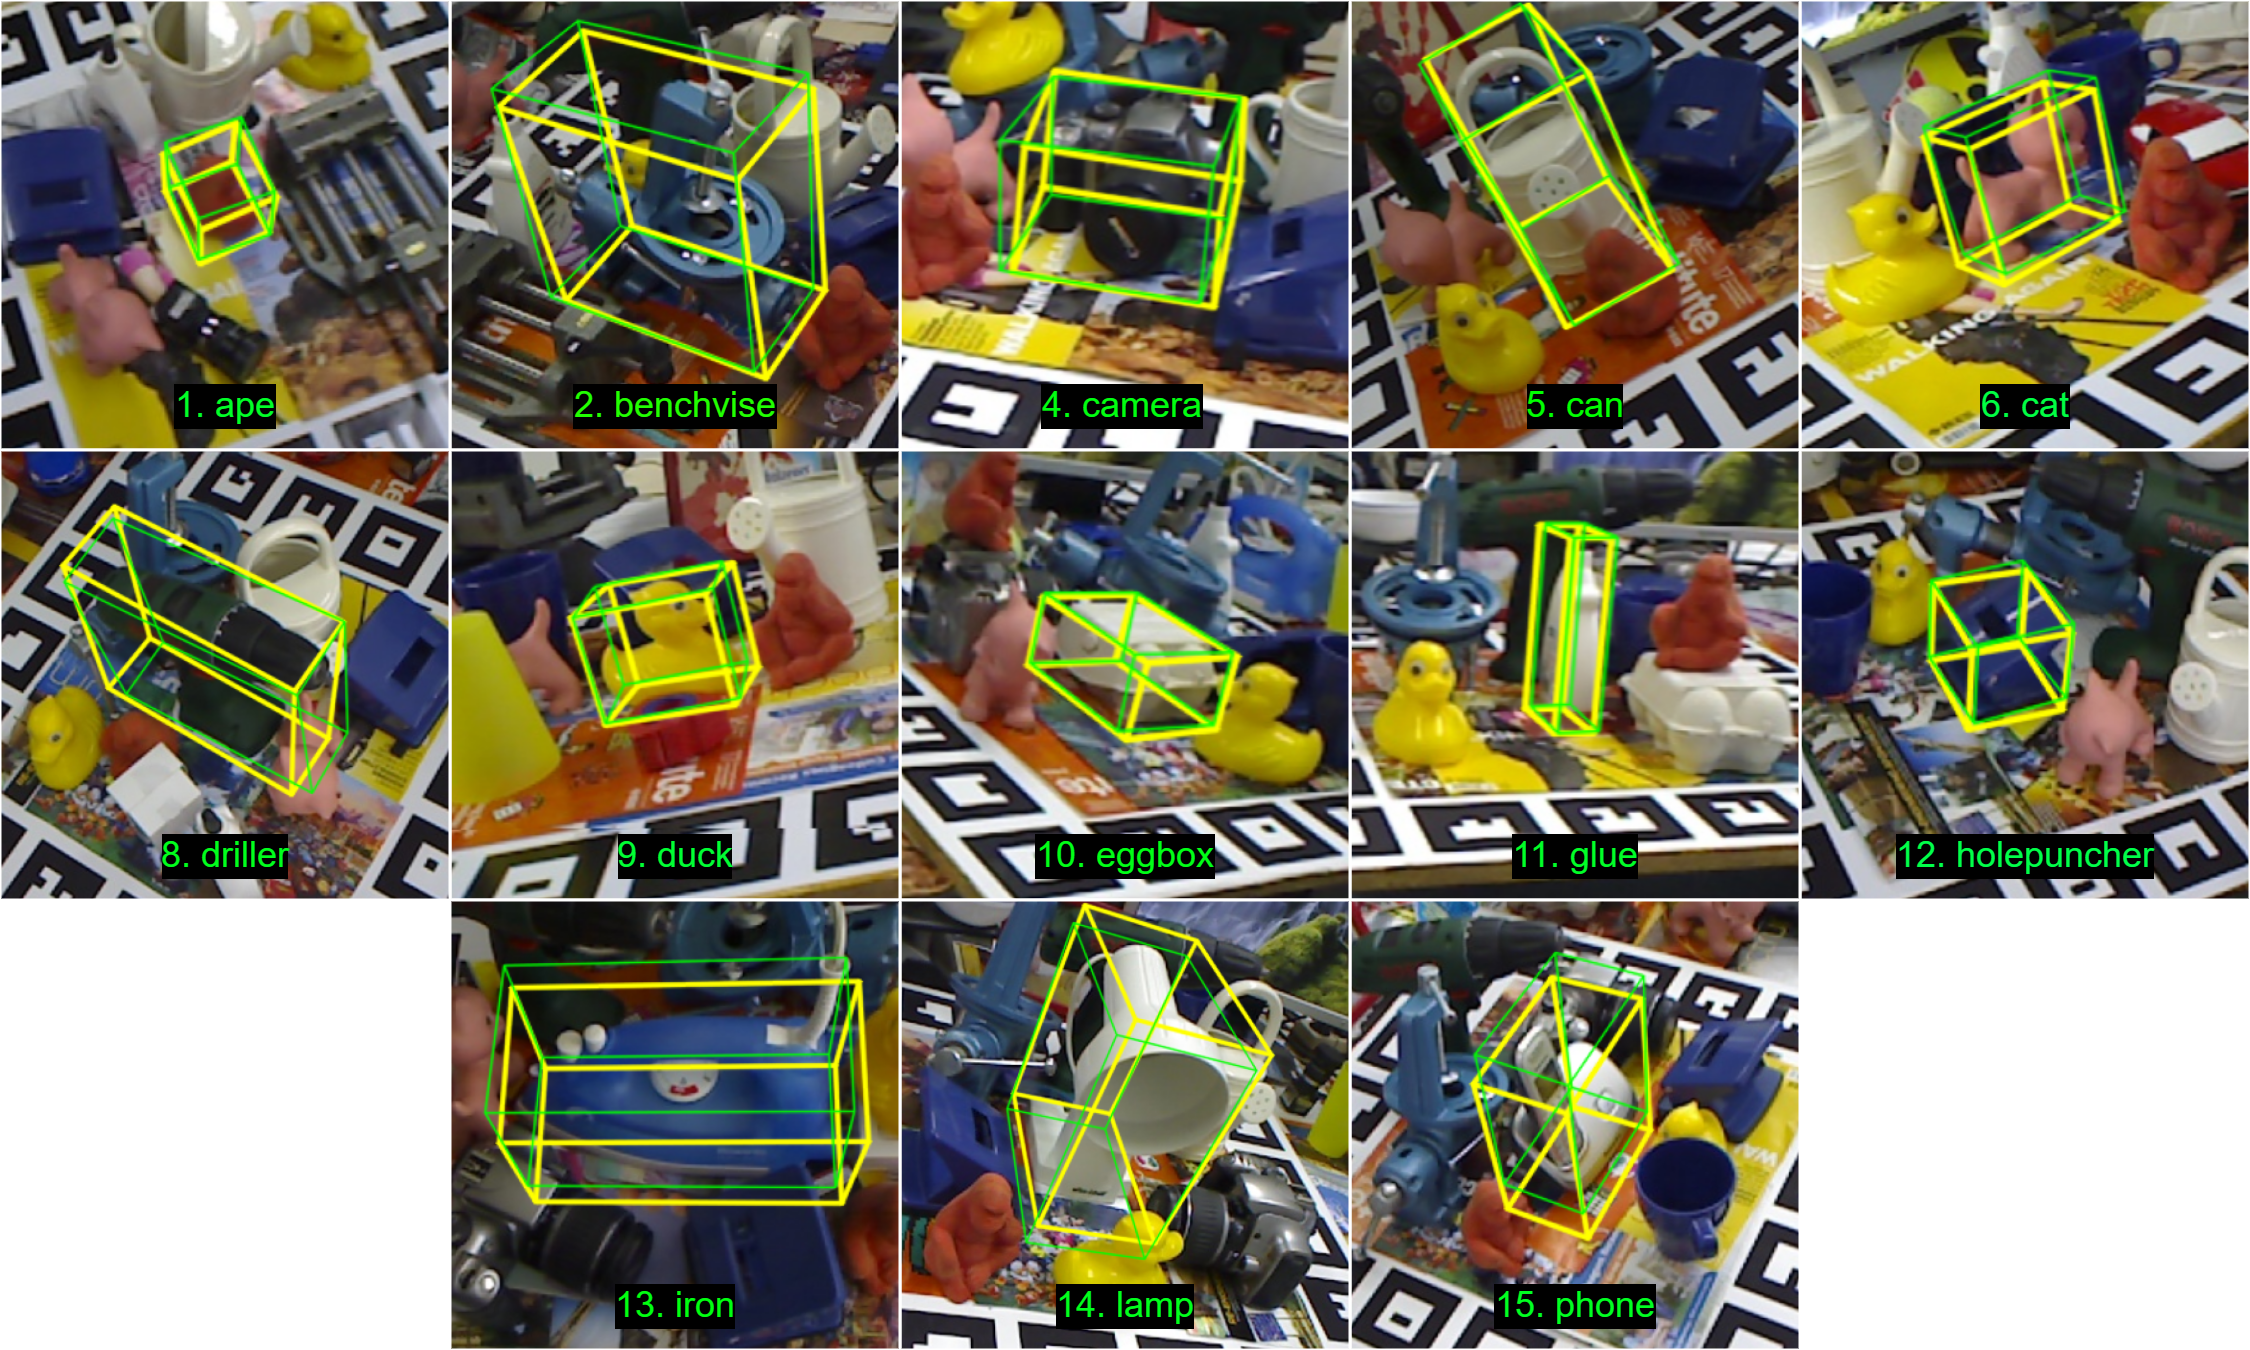
\includegraphics[width=\textwidth]{sec/figures/all-obj.png}
    \caption{Qualitative results showing predicted 3D bounding boxes (yellow) vs ground truth (green) for all 13 LineMOD objects.}
    \label{fig:qualitative}
\end{figure*}

\textbf{RGB vs RGB-D Gap:} The 43\% accuracy gap between RGB (41.2\%) and RGB-D (84.9\%) highlights the fundamental difficulty of monocular depth estimation. The RGB model must infer depth purely from appearance, while the RGB-D model benefits from direct geometric measurements.

\textbf{Challenging Objects:} Iron remains the most difficult object (48.7\% accuracy) due to its reflective surface that degrades both appearance features and depth sensor readings. Benchvise, driller, and phone also show lower accuracy (68-70\%), likely due to their larger size and complex geometry requiring more precise depth estimation.

\textbf{Symmetric Objects:} The ADD-S metric appropriately handles eggbox and glue, which achieve 100\% accuracy with RGBD. Without ADD-S, these objects would show artificially high errors due to equivalent rotations being penalized.

\textbf{Practical Implications:} Our results suggest that for applications requiring more than 80\% accuracy, depth sensors are essential. However, the RGB model (41.2\%) may suffice for coarse manipulation tasks or as a fallback when depth is unavailable.
